%-----------------------------------------------%

% PREAMBLE %

%-----------------------------------------------%
\documentclass[a4paper,12pt]{article}

% Packages
\usepackage{graphicx}
\usepackage{booktabs}
\usepackage{array}
\usepackage{amsmath, amssymb, amsthm}
\usepackage{geometry}
\usepackage{fancyhdr}
\usepackage{setspace}
\usepackage{titlesec}  % For title formatting
\usepackage{tocloft}
\usepackage{pgfplots}
\usepackage{xcolor}
\usepackage{enumitem}
\usepackage{graphicx, float}
\graphicspath{{LabReport4/}}


% Header and Footer
\pagestyle{fancy}
\fancyhf{}
\fancyhead[L]{Abereni Opuiyo}
\fancyhead[C]{PHY121}
\fancyhead[R]{\thepage}
\fancyfoot[L]{Lab Report 4: Free Fall}
\fancyfoot[R]{\thepage}
\geometry{margin=1.2in}
\setstretch{1.5}
\renewcommand{\footrulewidth}{0.1pt}% default is 0pt

% Table of Contents
\renewcommand{\contentsname}{Table of Contents}
\renewcommand{\cftsecleader}{\cftdotfill{\cftdotsep}}



% Title Formatting
\titleformat{\section}{\normalfont\Large\bfseries}{\thesection}{1em}{}


% Cover Page
\title{
    \vspace{5cm} % Adjust vertical space
    
\includegraphics[width=0.55\textwidth]{dutchess-logo-blue.png} \\ % Add your logo here (change "logo.png" to the actual filename)
    \vspace{1cm} % Adjust vertical space after the logo
    \textbf{\Huge Lab Report 4: Free Fall} \\
    \vspace{1cm} % Adjust vertical space
    \large PHY121 \\
    \vspace{0.5cm} % Adjust vertical space
    \large	October, 3rd, 2024 \\ 
		\vspace{.5cm}
		\large Professor R. Lathrop | Professor T. Zito
}
\author{Abereni Opuiyo}
\date{}
%-----------------------------------------------%

% TITLE PAGE %

%-----------------------------------------------%
\begin{document}
\maketitle
	\thispagestyle{empty}
\newpage

%-----------------------------------------------%

% Table of Contents  %

%-----------------------------------------------%
% Start page numbering from the Table of Contents

\setcounter{secnumdepth}{0}
\setcounter{page}{1}  % Start counting from 1
\tableofcontents
	\thispagestyle{fancy}
\newpage

%-----------------------------------------------%

% Purpose  %

%-----------------------------------------------%

\section{Purpose}
\vspace{-0.5cm}
\singlespacing
The purpose of this lab was to measure the acceleration due to gravity by dropping an object through a timer and recording its motion.Using the data we collected, we determined the approximate rate at which the object's velocity changed in the air.

%-----------------------------------------------%

% Theory  %

%-----------------------------------------------%

\section{Theory}
\vspace{-0.5cm}
\singlespacing

\indent If \textit{velocity} is the rate \& direction of an object's \textit{position} over a certain time interval, then \textit{acceleration} is the rate \& direction of an object's \textit{velocity} over a certain time interval. So long as an object's velocity is changing, it has acceleration.\par 


Velocity and acceleration are both \textit{vector} quantities, meaning both have vertical and horizontal components. The vertical component of an object's acceleration is impacted by the Earth's gravity. The acceleration due to gravity on Earth's surface has been measured to be \textit{$9.80\thinspace{m/s^2}$}. \par

\begin{figure}[h!]
    \centering
    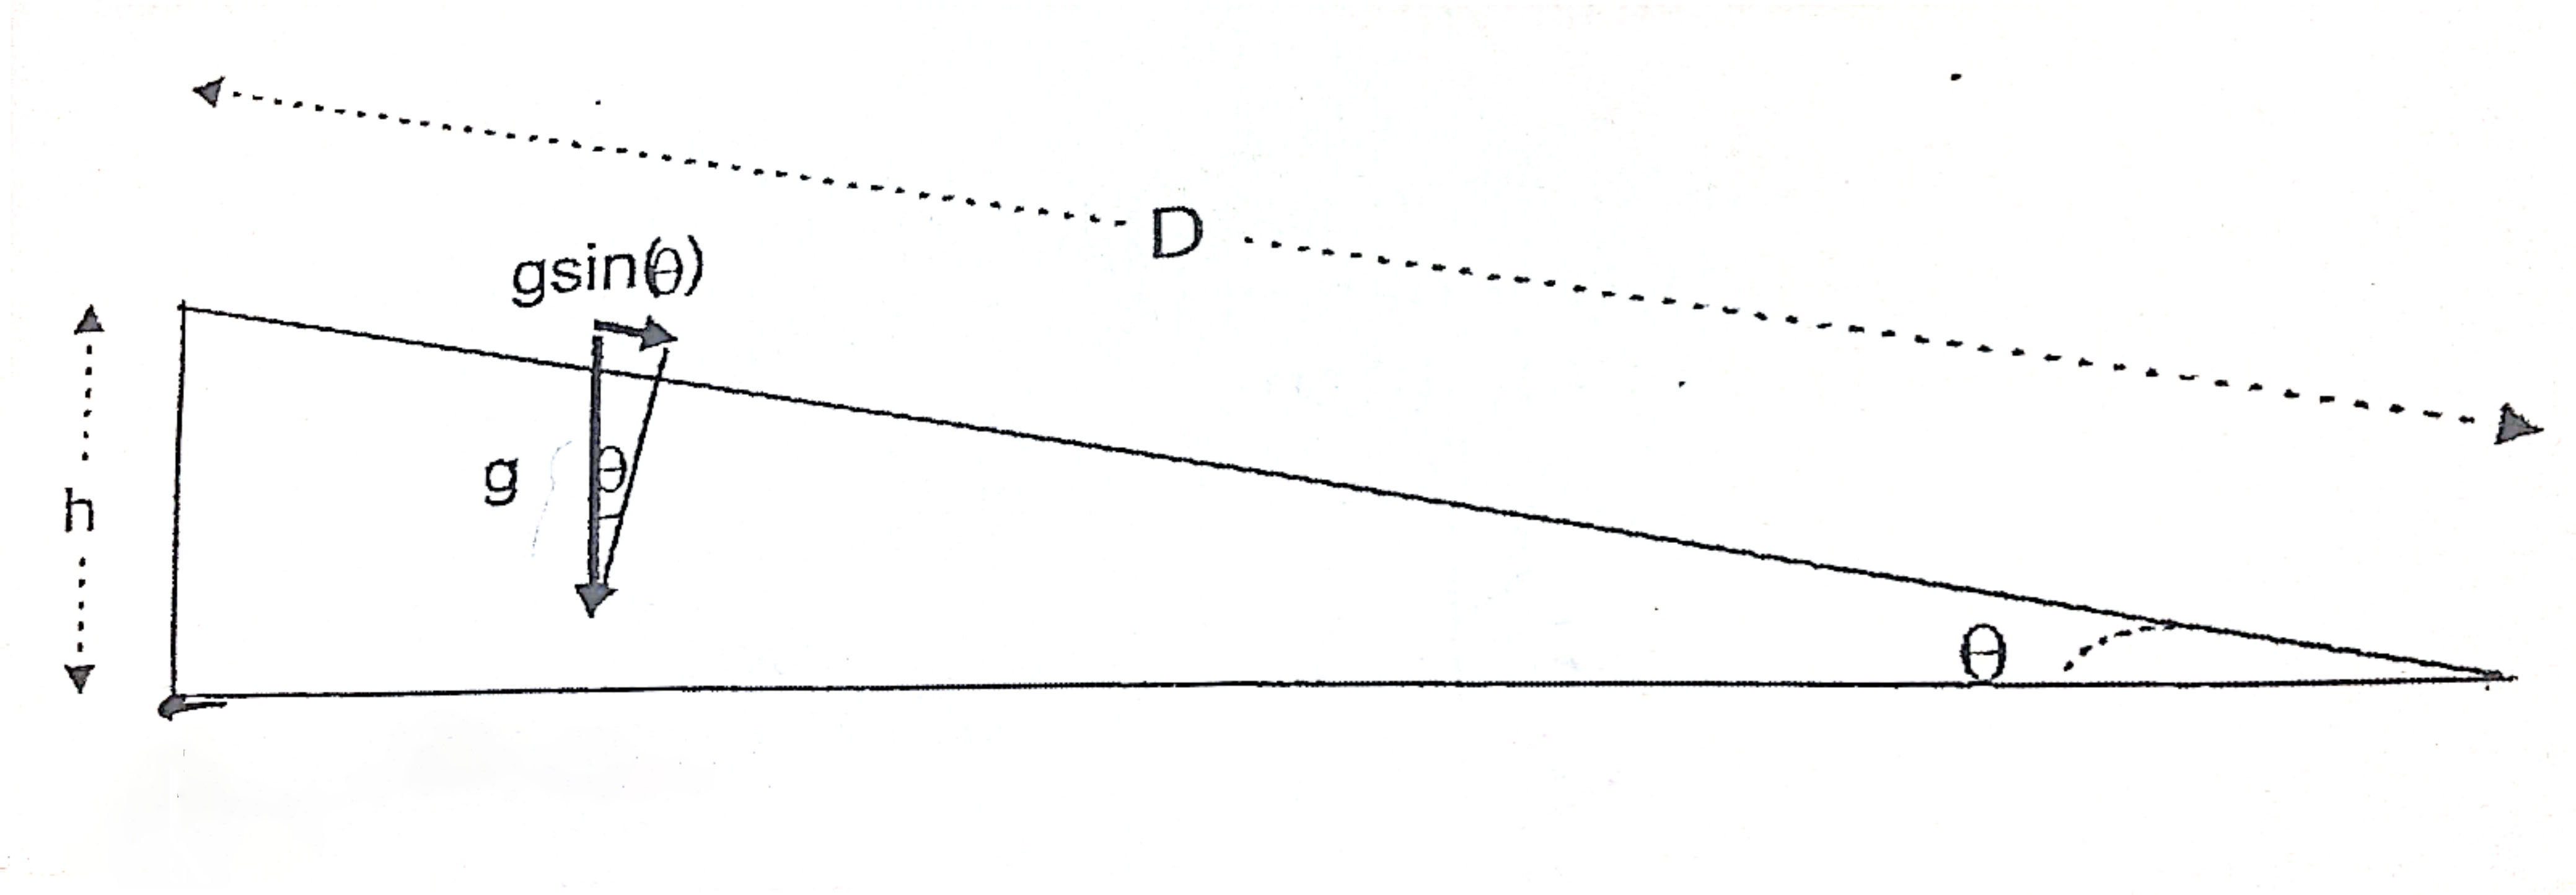
\includegraphics[width=0.8\textwidth]{figure1_inclineplane} % Example of adding a figure
    \caption{Incline plane}
    \label{fig:inclineplane}
\end{figure}

When objects fall straight down, assuming there's no air resistance, the vertical component of the object's acceleration is simply $9.80\thinspace{m/s^2}$. However, if the object is launched at an angle, then the object's acceleration in the vertical direction must be determined in a different way. Just as one would determine the horizontal \& vertical components of velocity for objects thrown at angles using trigonometric functions, so too can the acceleration due to gravity of such objects be calculated. More specifically, for objects that move along \textit{inclined planes} (see figure \ref{fig:inclineplane}), the component of the acceleration vector parallel to the plane can be calculated with the following equation:

\begin{equation}
a = gsin\theta
\label{eq:1}
\end{equation}

The plane angle (figure \ref{fig:inclineplane}) can be determined using:

\begin{equation}	
sin\theta = \frac{\Delta{h}}{D}
\label{eq:2}
\end{equation}

\newpage


%-----------------------------------------------%

% Procedure  %

%-----------------------------------------------%


\section{Procedure}
\vspace{-0.5cm}
\singlespacing


%Free Fall

\subsection{Free Fall}

\subsubsection{Setup}

	\begin{enumerate}

		\item Plugged in \textbf{Accessory Photogate Timer} into Ch. 1 on \textbf{Lab Pro} interface
		\item Opened \textbf{Logger Pro}
			
		\item Tested sensor by pressing \textit{"collect"} on \textbf{Logger Pro}
	\end{enumerate}	

\subsubsection{Measure Times \& Find Acceleration}
	\begin{enumerate}[resume]

		\item Dropped \textbf{picket fence} vertically through \textbf{Photogate Timer}
	
		\item Recorded data from \textit{Velocity vs Time} plot

		\item Calculated slope of velocity by hand and record your calculations

		\item Used the linear regression function on \textbf{Logger Pro} to find the average velocity of the object

		\item Saved graph of acceleration

		\item Repeated steps 4-5, five more times and recorded the average acceleration of the trials
	\end{enumerate}

\subsection{Inclined Plane}

\subsubsection{Setup}

	\begin{enumerate}
		\item Connected \textbf{Motion Detector} to \textbf{Lab Pro} 
		\item Tested sensor by pressing \textit{"collect"} on \textbf{Logger Pro}
		\item Placed sensor at bottom of track
		\item Used a \textbf{meter stick} to measure 0.40\thinspace m of distance between the motion sensor and the cart and marked it.
	\end{enumerate}

\subsubsection{Starting at the Top}

	\begin{enumerate}[resume]

	\item Held cart at marked spot and released it
	\item Recorded average acceleration of linear region in the data using linear fit function in \textbf{Logger Pro}
	\item Repeated steps 5-6 another three times 
	\item Calculated and recorded average acceleration of cart during the four trials
	\item Used \textbf{meter stick} to measure D and h of the track as described in figure \ref{fig:inclineplane} to calculate angle of track using equation \eqref{eq:2}
	\item Calculated difference between average acceleration in trials and acceleration from equation \eqref{eq:2}
	\end{enumerate}

	\subsubsection{Starting at the Bottom}

	\begin{enumerate}[resume]
			\item Practiced pushing cart up track at least 0.40\thinspace m from the motion sensor
			\item Recorded motion of track when moving from the bottom and calculated its acceleration.
			\item Repeated and recorded motion trial three more times, then calculated average acceleration
		\end{enumerate}


%-----------------------------------------------%

		% Calculations & Graph   %

%-----------------------------------------------%


\section{Calculations \& Graphs}

\vspace{-0.5cm}
\singlespacing

%------- AVERAGE VALUE --------%

\subsection{Average Value Formula} 

\begin{align*}
		\overline{a} = \frac{sum\,of\,values}{total\, \#\,of\,values} 
\end{align*}

\subsubsection{Sample Calculation \\ {\normalfont \small\textit{average acceleration of free fall trials}}}

\begin{align*}
	\overline{a} & = \frac{9.751 + 9.758 + 9.749 + 9.620 + 9.769 + 9.837}{6} \\
							 &= \boxed{9.747\thinspace m/s^2}
\end{align*}

%------- AVERAGE VALUE --------%

%------- STANDARD DEVIATION --------%
\subsection{Standard Deviation Formula}

\begin{align*}
		\sigma &= \sqrt{\frac{\Sigma(x_i -\overline{a})^2}{N}} \\
		 &= \sqrt{\frac{SS}{N}} \\ \\
		\textbf{N} &:\, \text{Total number of values} \\
		\overline{\textbf{a}} &:\, \text{Average value} \\
		\textbf{x\textsubscript{i}} &:\, \text{Each value from the data set} \\
		\textbf{SS} &:\, \text{Sum of squares} 
\end{align*}

\subsubsection{Sample Calculation \\ {\normalfont \small\textit{std of free fall trials}}}

\begin{align*}
	\sigma &= \sqrt{\frac{(9.751-\overline{a})^2 + ... + (9.837-\overline{a})^2}{6}} \\
		 &= \sqrt{\frac{0.024865333}{6}} \\
		 &= \boxed{0.06439\thinspace m/s^2}
\end{align*}
%------- STANDARD DEVIATION --------%

%------- RELATIVE ERROR --------%
\subsection{Relative Error Formula}

\begin{align*}
	RE &= \left| {\frac{V_A-V_E}{V_E}} \right|\: \text{x}\: 100\% \\ \\
	\boldsymbol{V_A} &:\, \text{Actual value observed} \\
	\boldsymbol{V_E} &:\, \text{Expected value} 
\end{align*}

\subsubsection{Sample Calculation \\ {\normalfont \small\textit{acceleration of free fall trial 1}}}

\begin{align*}
	RE &= \left| {\frac{9.751-9.80}{9.80}} \right|\: \text{x}\: 100\% \\
			&= \boxed{0.4917\%} 
\end{align*}
%------- RELATIVE ERROR --------%

\subsection{Free Fall}

\subsubsection{Trial 1}
%----FF TRIAL 1-----%
\begin{table}[H]
\centering
\begin{tabular}{@{}cc@{}}
\toprule
\textbf{Time(s)} & \textbf{Velocity(m/s)} \\ \midrule
0.0532 & 1.199 \\
0.08952 & 1.553 \\
0.1189 & 1.841 \\
0.1444 & 2.087 \\
0.1671 & 2.31 \\
0.1878 & 2.513 \\ \midrule
\textbf{\begin{tabular}[c]{@{}c@{}}Average \\ Acceleration \\ ($\boldsymbol{m/s^2}$)\end{tabular}} & 9.751 \\ \bottomrule
\end{tabular}
\caption{Velocity vs Time | Free Fall Trial 1}
\label{tab:ff-t1}
\end{table}

\begin{figure}
	\begin{center}
		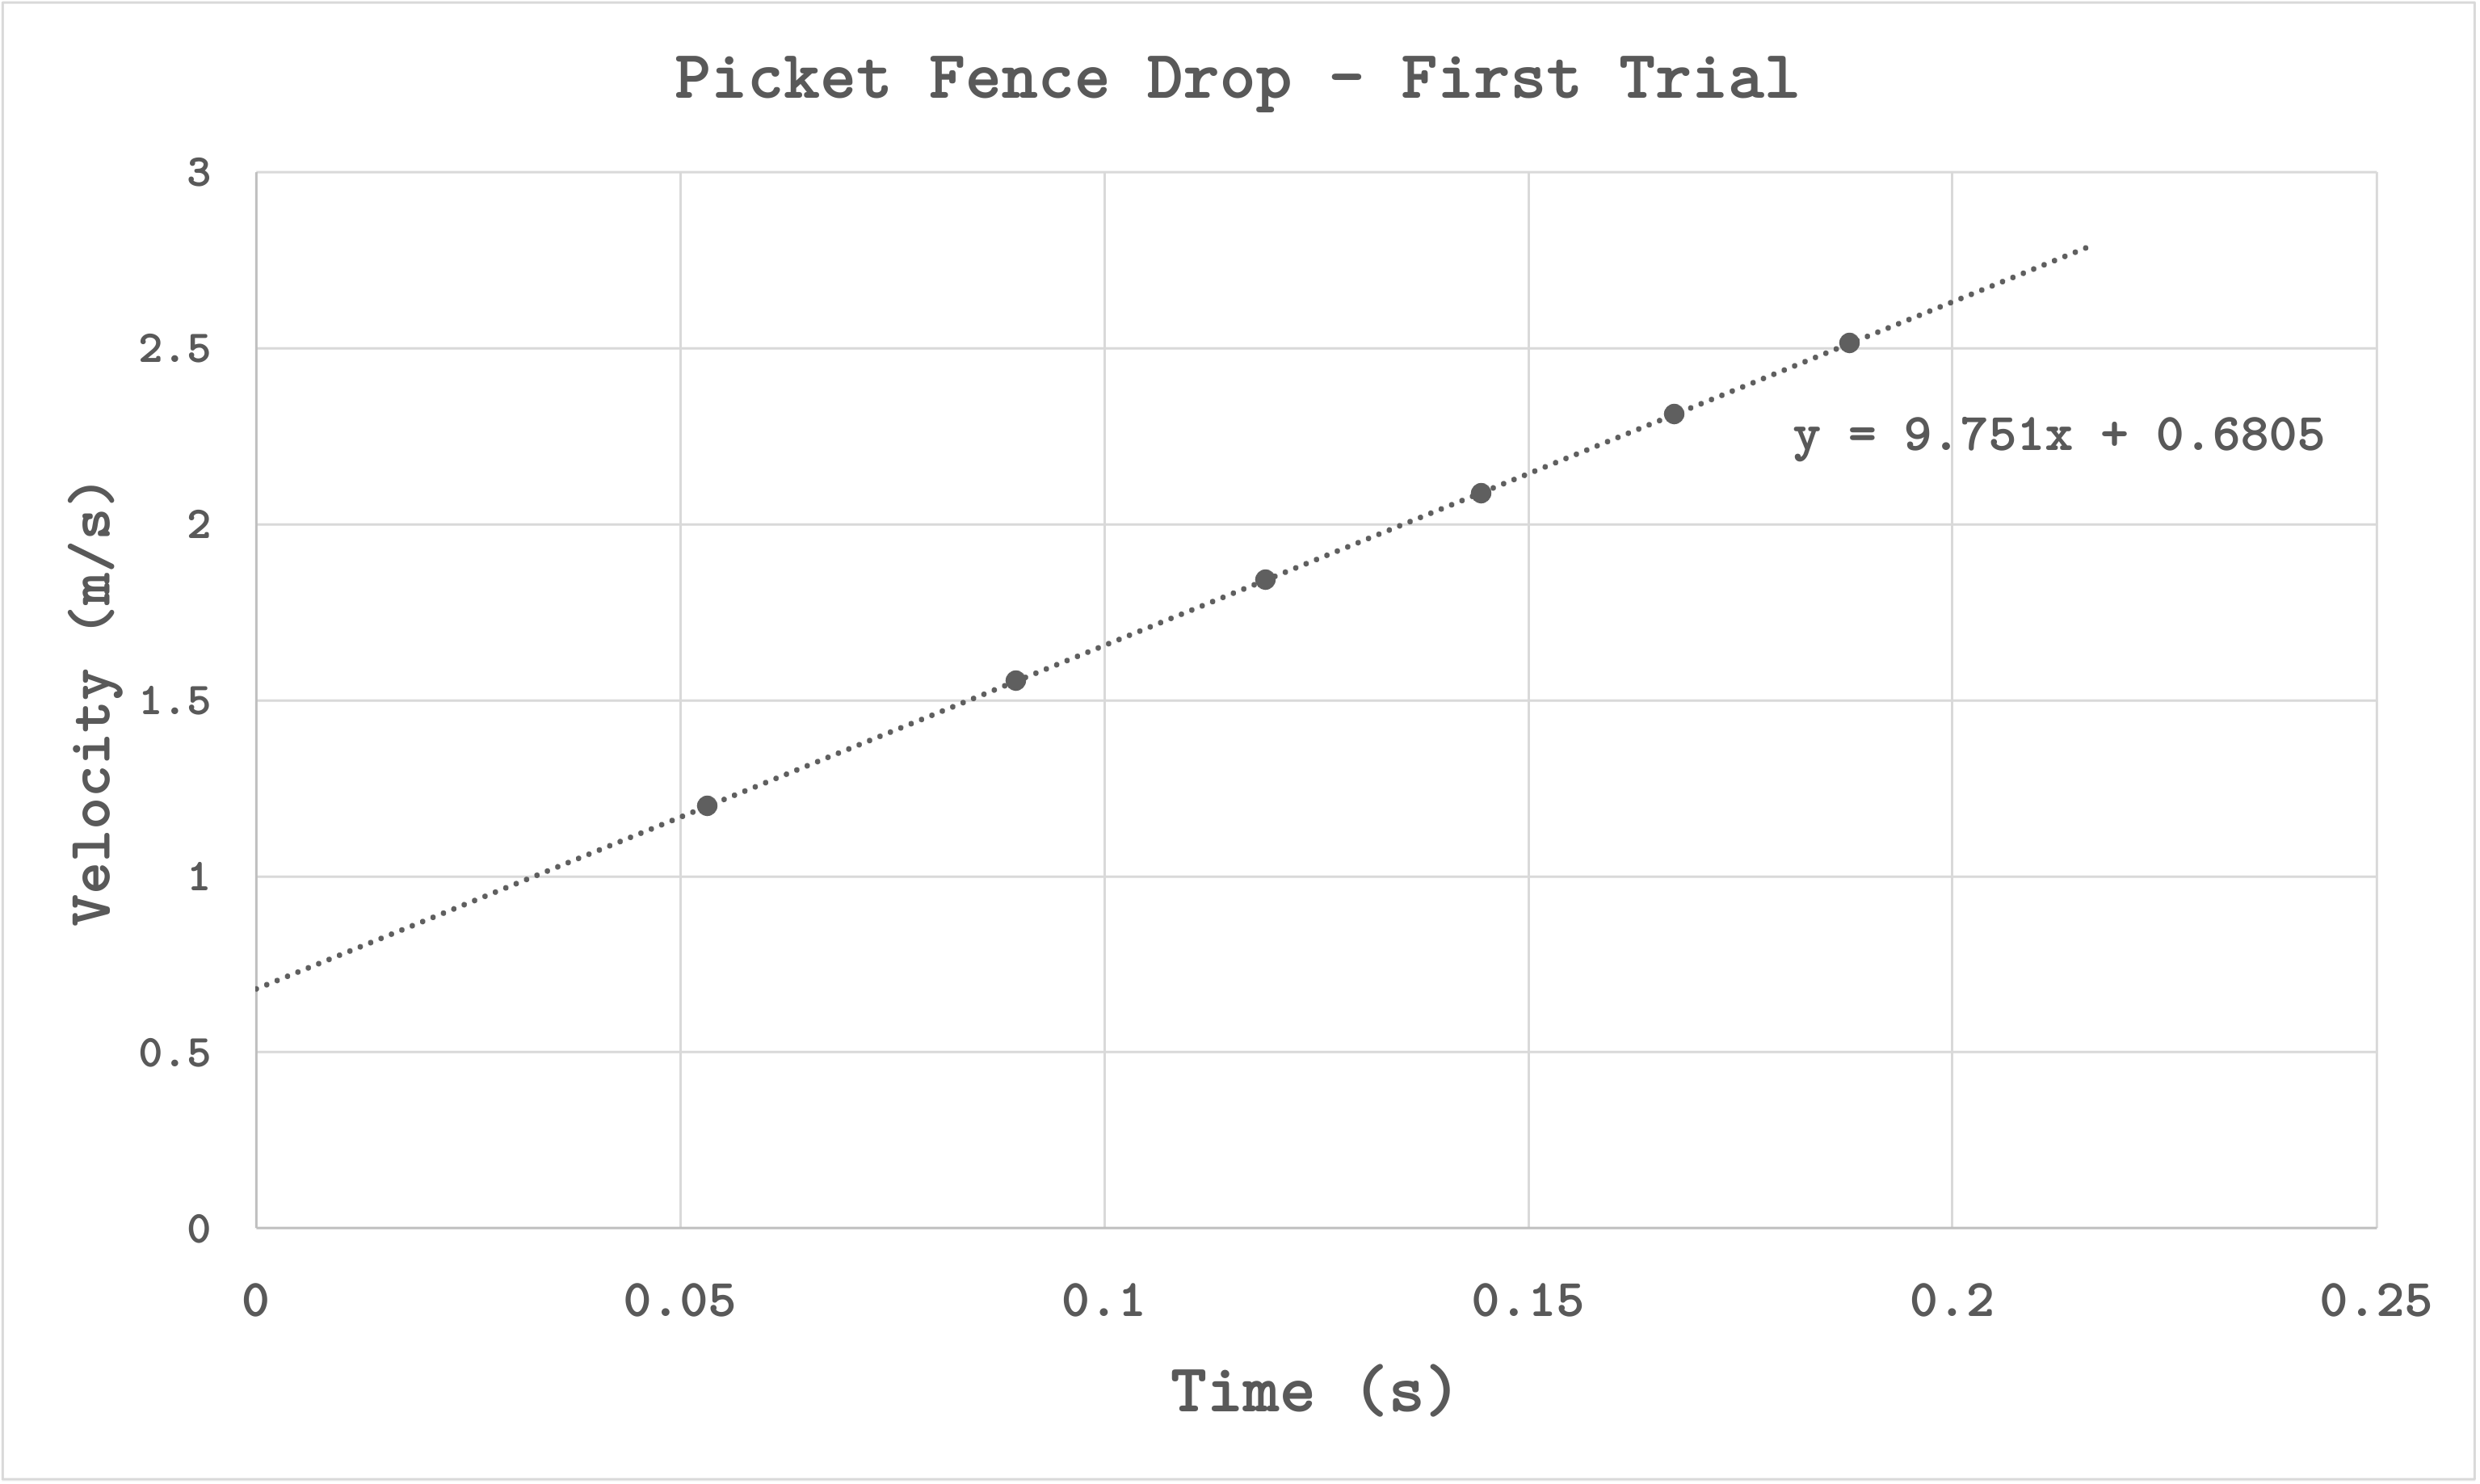
\includegraphics[width=0.95\textwidth]{picket1.png}
	\end{center}
	\caption{Velocity vs Time Graph | Free Fall Trial 1}
	\label{fig: picketg1}
\end{figure} 

%----FF TRIAL 1-----%

%----FF TRIAL 1-6-----%
\subsubsection{Trials 1-6}

\begin{table}[H]
\centering
\begin{tabular}{@{}ccc@{}}
\toprule
\textbf{Trials} & \textbf{Acceleration} & \textbf{Relative Error (\%)} \\ \midrule
1 & 9.751 & 0.4917 \\
2 & 9.758 & 0.4271 \\
3 & 9.749 & 0.5108 \\
4 & 9.62 & 1.829 \\
5 & 9.769 & 0.3135 \\
6 & 9.837 & 0.3877 \\ \midrule
\textbf{Average ($\boldsymbol{m/s^2}$)} & 9.747 &  \\
\textbf{Standard Deviation ($\boldsymbol{m/s^2}$)} & 0.06439 &  \\ \bottomrule
\end{tabular}
\caption{Free Fall Acceleration | Trials 1-6}
\label{tab:ff-ta}
\end{table}
%----FF TRIAL 1-6-----%

\subsection{Inclined Plane}

%----ACCELERATION VECTOR AND ANGLE-----%

	\subsubsection{Plane Angle}
	\begin{align*}
		sin\theta &= \frac{\Delta h}{D} \\
		\boldsymbol{\Delta h} &: \text{height of the track at two points} = \boxed{.01870\,m} \\
		\textbf{D} &: \text{distance along the track between two points} = \boxed{.3\,m} \\
		sin\theta &= 0.0623 = \boxed{3.57^\circ}
	\end{align*}

	\subsubsection{Acceleration Vector on Incline Plane}
	
	\begin{align*}
		a&=gsin\theta \\
		\textbf{g} &: \text{Acceleration due to gravity on Earth} = \boxed{9.80\,m/s^2} \\
		\boldsymbol{sin\theta} &: \text{Angle of track} \\
		a&=gsin\theta = \boxed{-.6105\,m/s^2}
	\end{align*}
%----ACCELERATION VECTOR AND ANGLE-----%

%----STARTING FROM THE TOP TRIAL 1-----%
\subsubsection{Starting From The Top - Trial 1}
\begin{figure}[H]
	\begin{center}
		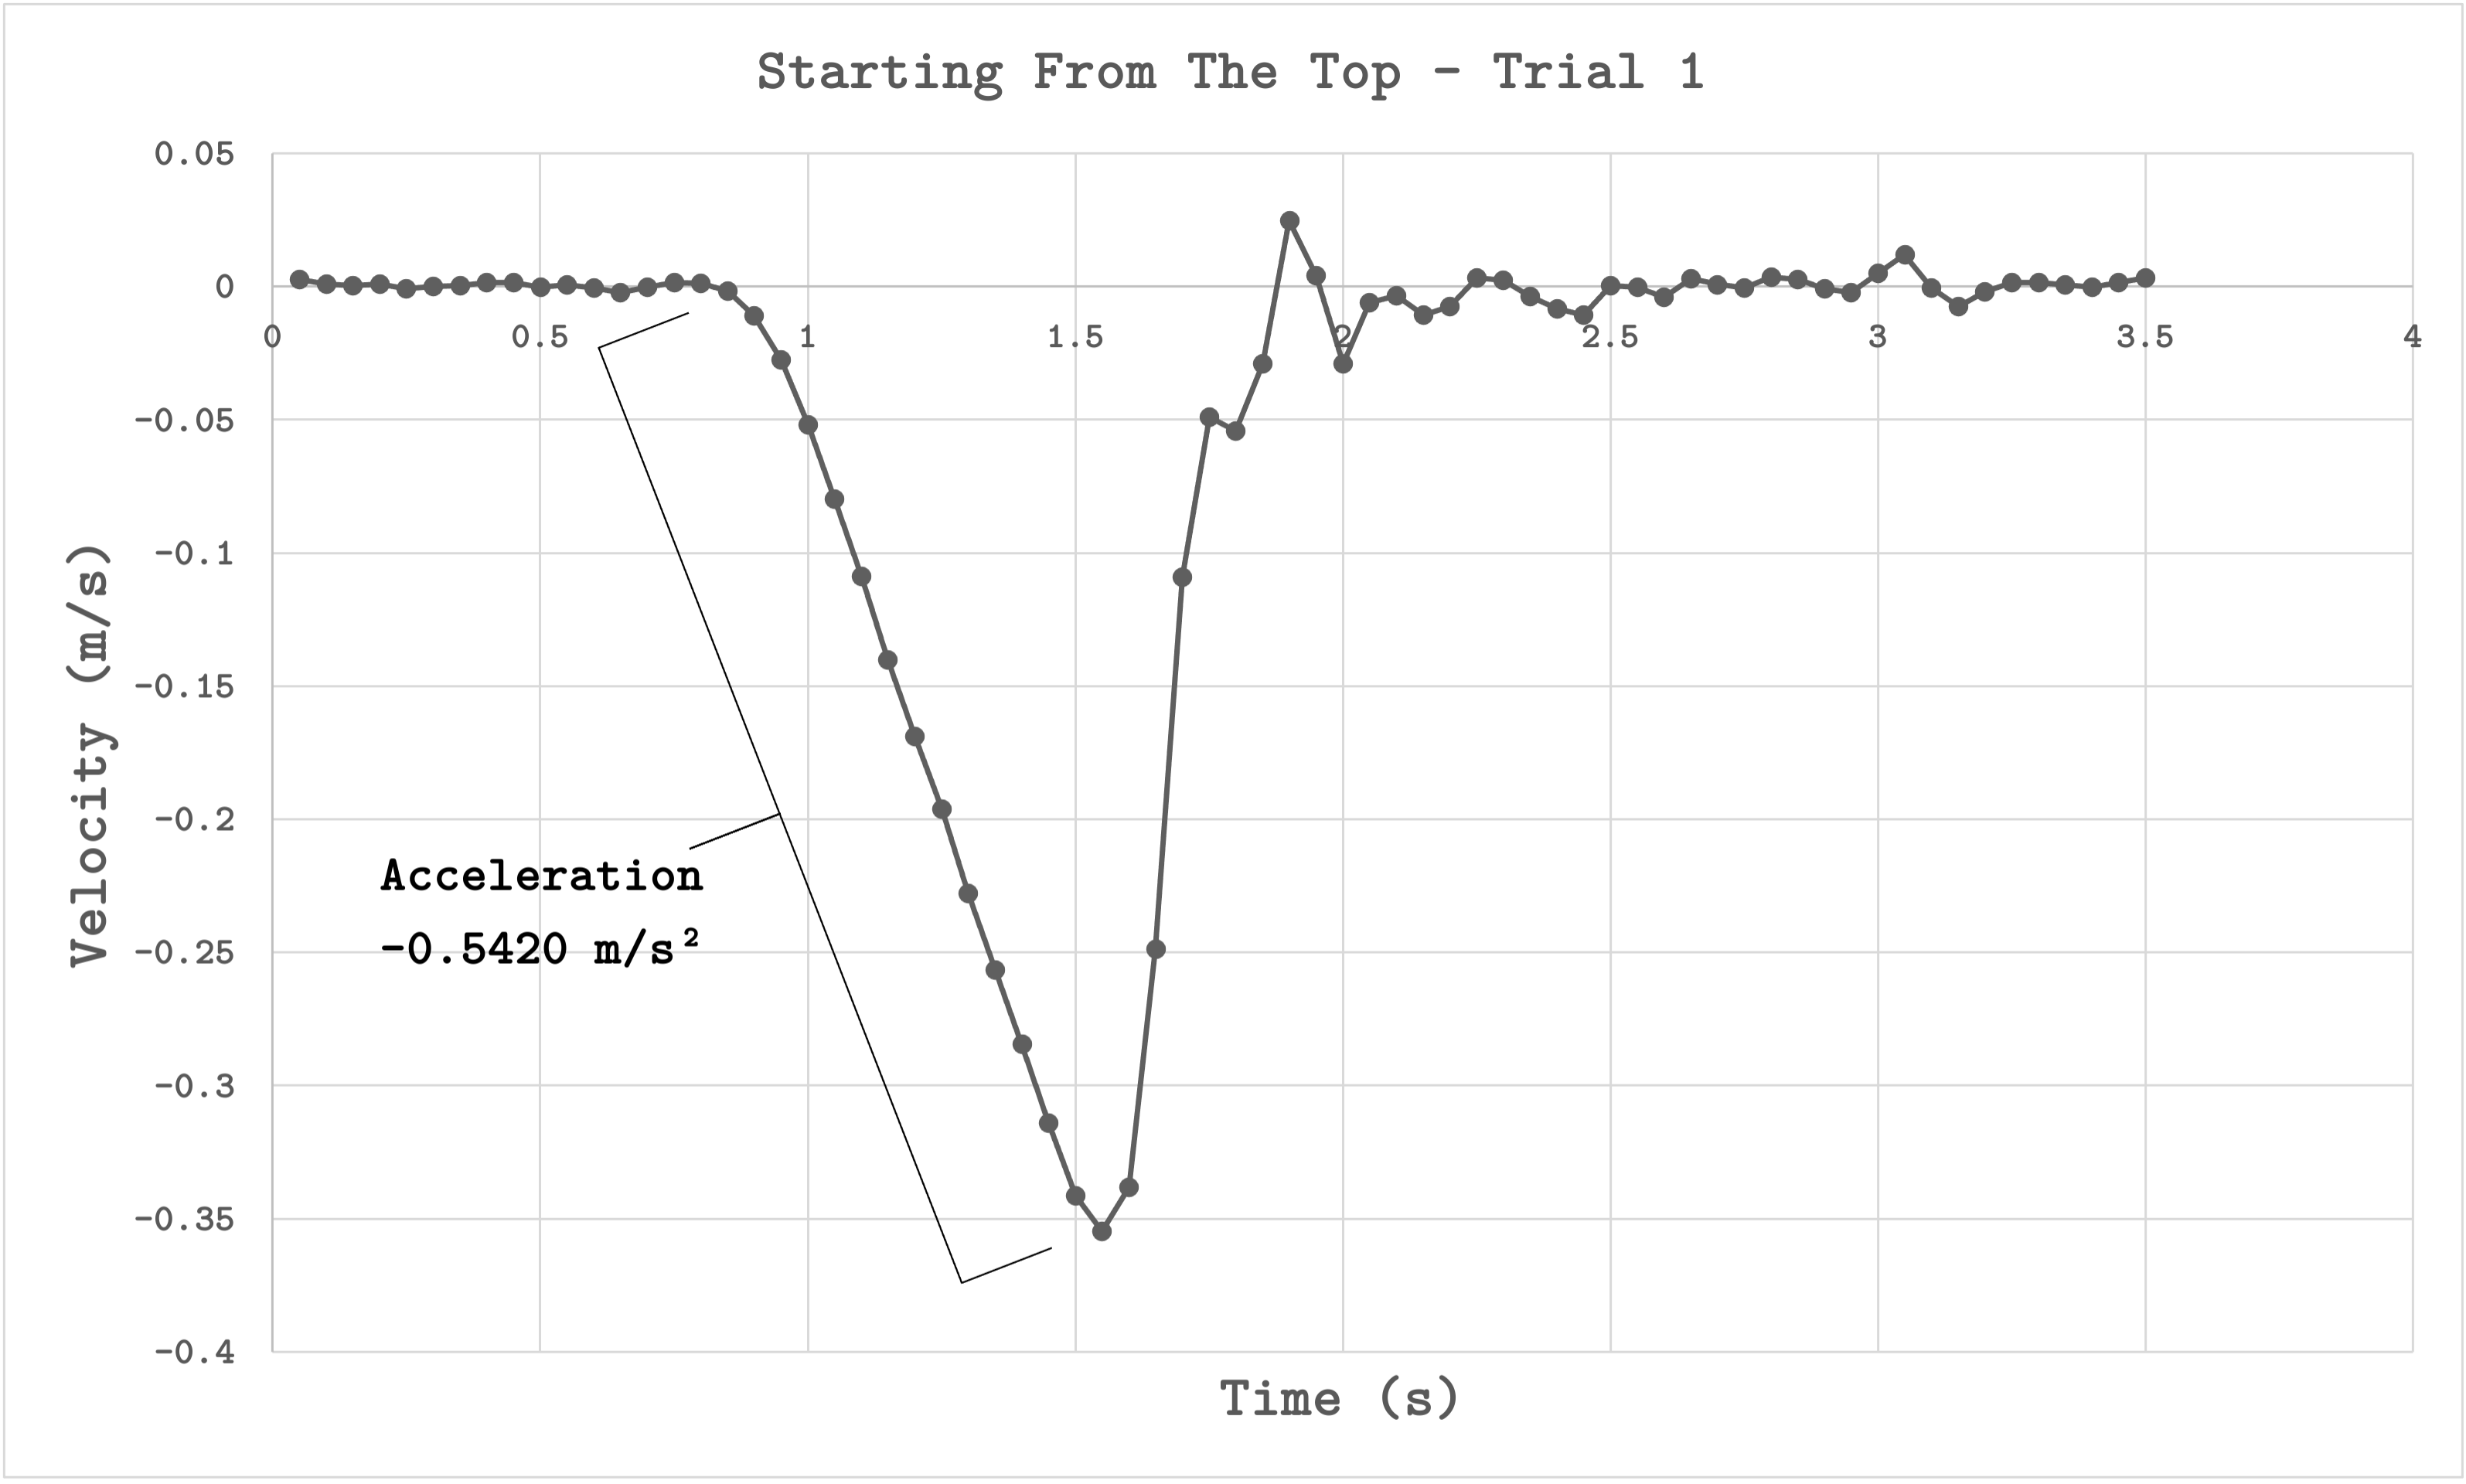
\includegraphics[width=0.95\textwidth]{cartg1.png}
	\end{center}
	\caption{Starting From The Top Graph | Trial 1}
	\label{fig: cartg1}
\end{figure} 
%----STARTING FROM THE TOP TRIAL 1-----%

%----STARTING FROM THE TOP TRIAL 1-4-----%
\subsubsection{Starting From The Top - Trials 1 - 4}

\begin{table}[H]
\centering
\begin{tabular}{@{}ccc@{}}
\toprule
\textbf{Trials} & \textbf{Acceleration} & \textbf{Relative Error (\%)} \\ \midrule
1 & -0.542 & 11.22 \\
2 & -0.5315 & 12.94 \\
3 & -0.529 & 13.34 \\
4 & -0.5244 & 14.1 \\ \midrule
\textbf{Average ($\boldsymbol{m/s^2}$)} & -0.5317 &  \\
\textbf{Standard Deviation ($\boldsymbol{m/s^2}$)} & 0.006455 &  \\ \bottomrule
\end{tabular}
\caption{Starting From The Top | Trials 1-4 }
\label{tab:ip-sftt}
\end{table}
%----STARTING FROM THE TOP TRIAL 1-4-----%

%----STARTING FROM THE BOTTOM TRIAL 1-----%
\subsubsection{Starting From The Bottom - Trial 1}
\begin{figure}[H]
	\begin{center}
		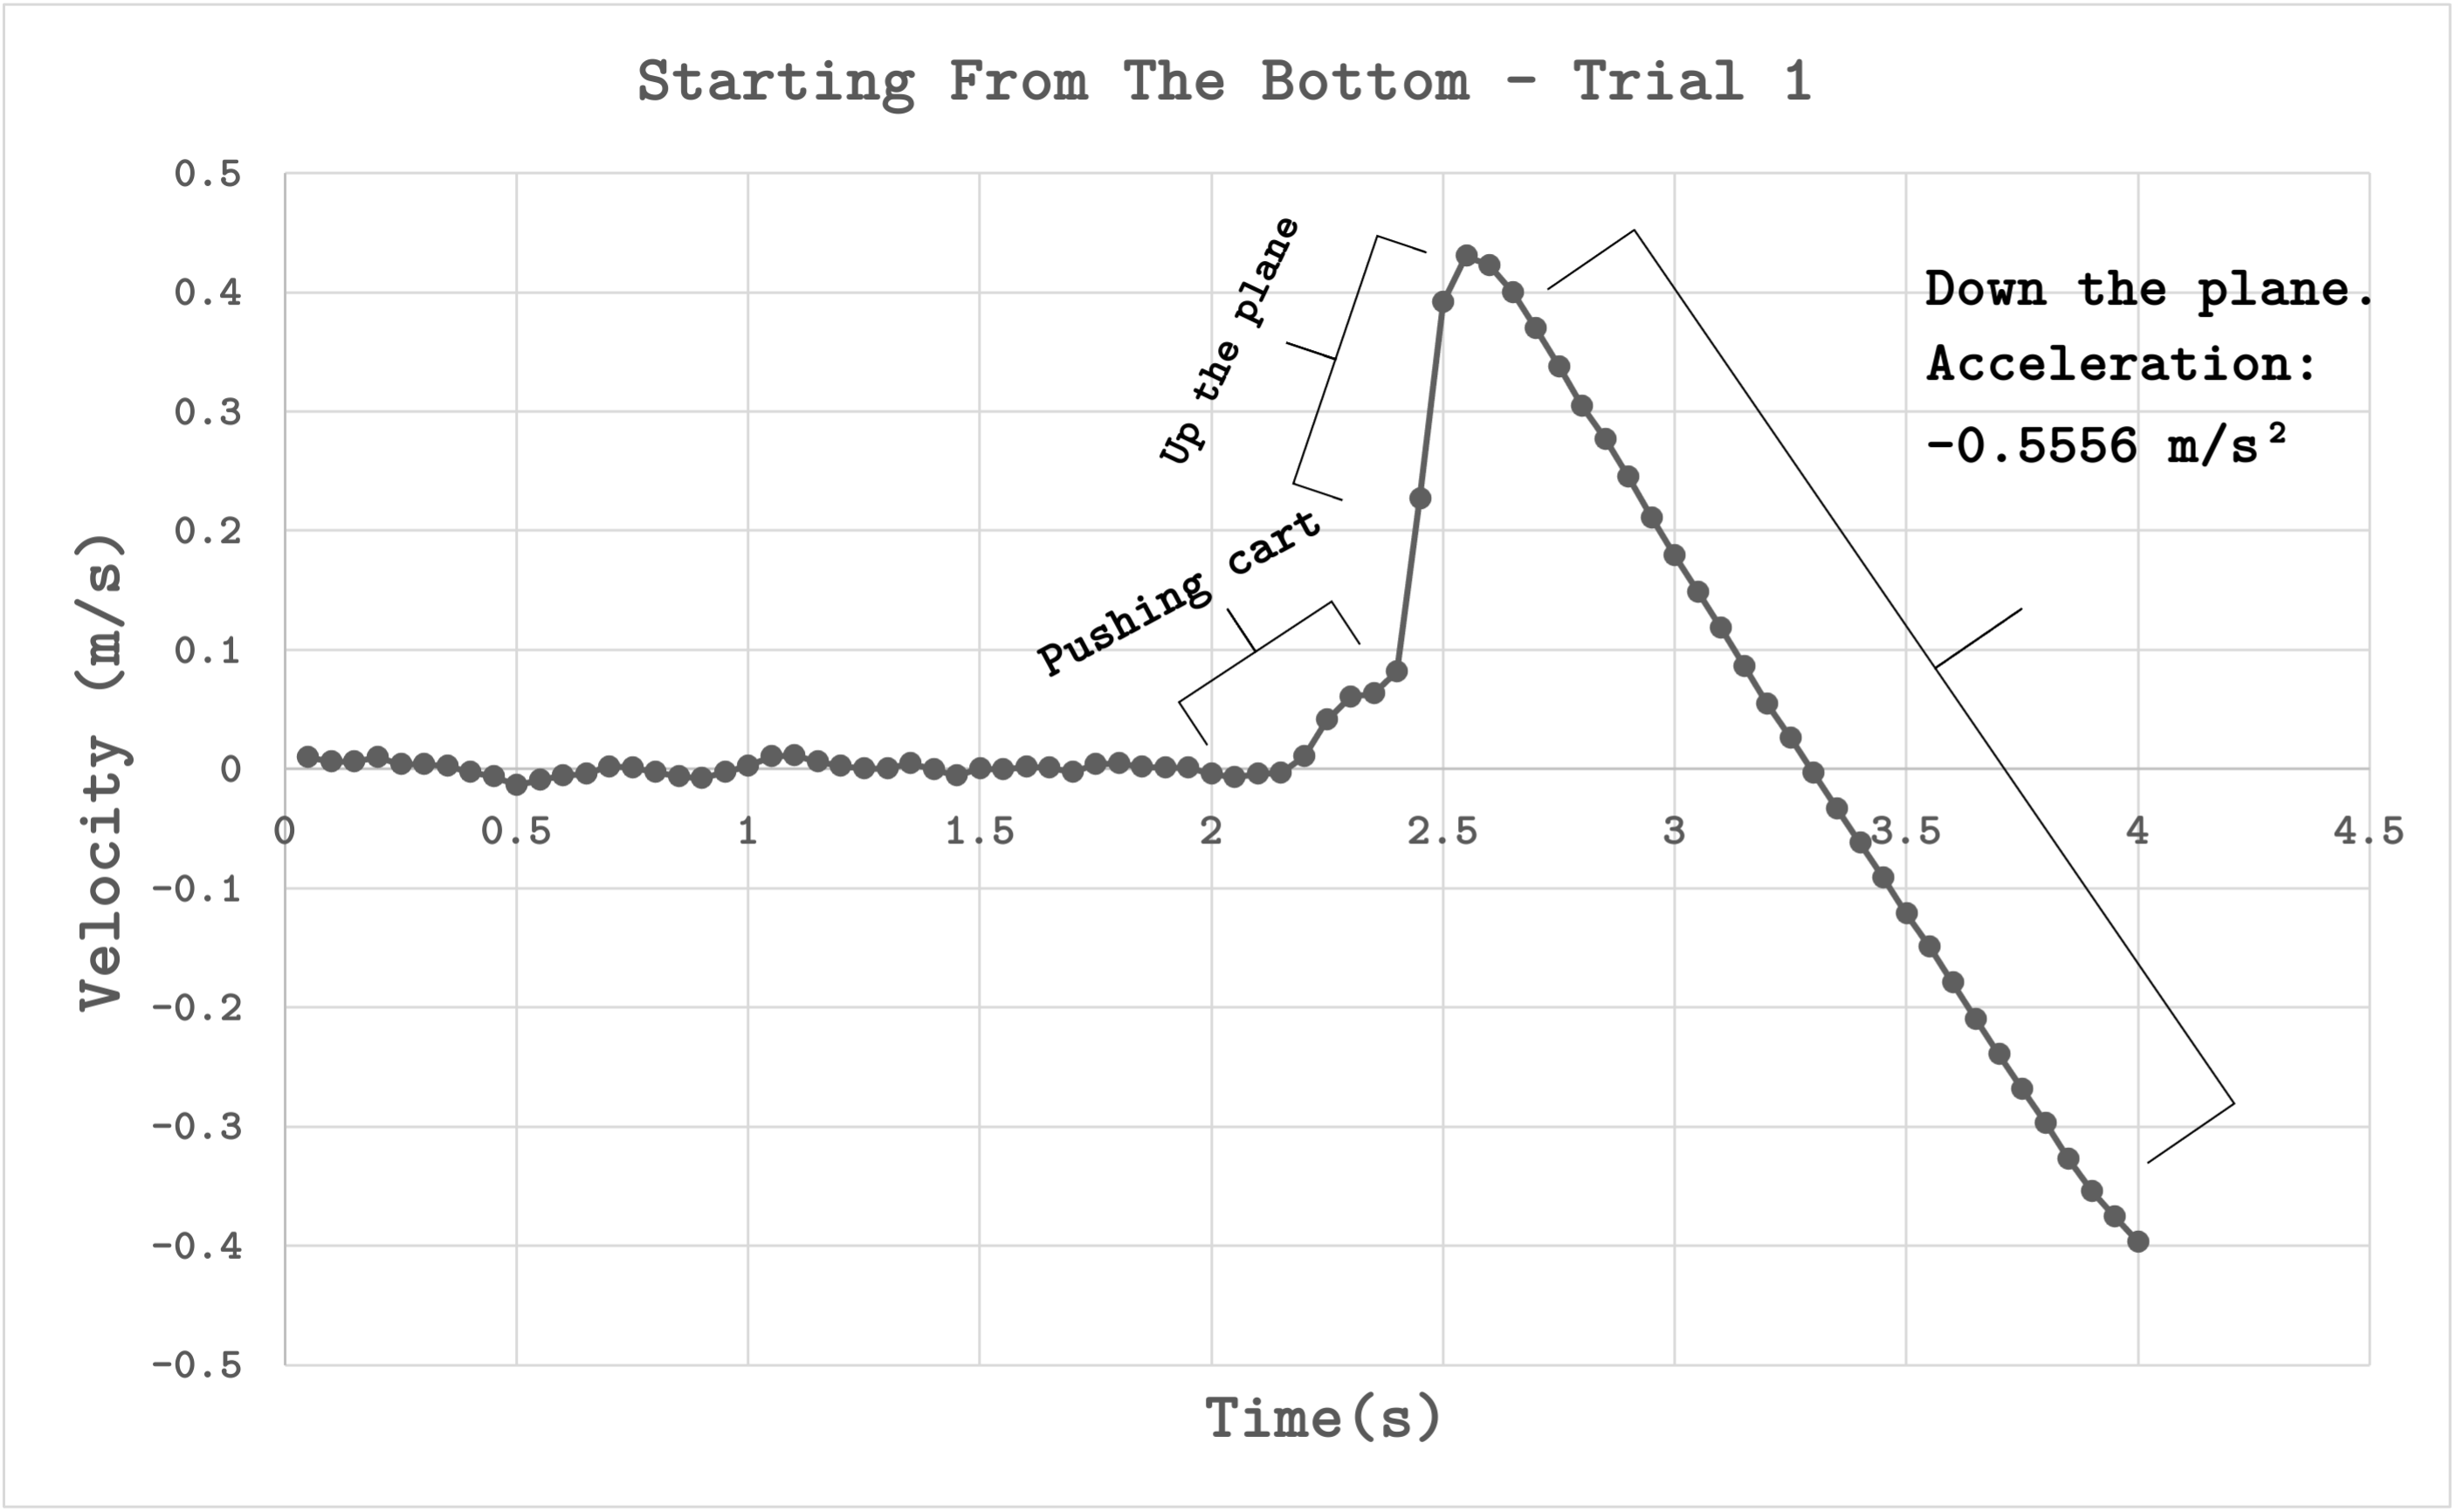
\includegraphics[width=0.95\textwidth]{cartg2.png}
	\end{center}
	\caption{Starting From The Bottom Graph | Trial 1}
	\label{fig: cartg2}
\end{figure} 

%----STARTING FROM THE BOTTOM TRIAL 1-----%

%----STARTING FROM THE BOTTOM TRIAL 1-4-----%
\subsubsection{Starting From The Bottom - Trials 1 - 4}

\begin{table}[H]
\centering
\begin{tabular}{@{}ccc@{}}
\toprule
\textbf{Trials} & \textbf{Acceleration} & \textbf{Relative Error (\%)} \\ \midrule
1 & -0.5556 & 8.992 \\
2 & -0.5755 & 5.733 \\
3 & -0.5622 & 7.911 \\
4 & -0.5639 & 7.633 \\ \midrule
\textbf{Average Acceleration ($\boldsymbol{m/s^2}$)} & -0.5643 &  \\
\textbf{Standard Deviation ($\boldsymbol{m/s^2}$)} & 0.007171 &  \\ \bottomrule
\end{tabular}
\caption{Starting From The Bottom | Trials 1-4}
\label{tab:ip-sftb}
\end{table}
%----STARTING FROM THE BOTTOM TRIAL 1-----%

%----INCLINE PLANE AVERAGES RE-----%
\subsubsection{Incline Plane Averages - Relative Error}
\begin{table}[H]
\centering
\begin{tabular}{@{}ccc@{}}
\toprule
 & \textbf{Acceleration ($\boldsymbol{m/s^2}$)} & \textbf{Relative Error (\%)} \\ \midrule
\textbf{SFTT} & -0.5317 & 12.9 \\
\textbf{SFTB} & -0.5643 & 7.567 \\ \bottomrule

\end{tabular}
\caption{Inclined Plane Averages | Relative Error}
\label{tab:ip-re}
\end{table}
%----INCLINE PLANE AVERAGES RE-----%

%-----------------------------------------------%

% Questions  %

%-----------------------------------------------%


 \section{Questions}

\vspace{-0.5cm}
\singlespacing

\begin{enumerate}
	\item \textbf{What do you expect the acceleration of the picket fence to be? Is it exactly this value? If yours is higher or lower provide explanations as to why that might be.}

		We expected the acceleration of the picket fence to be around $9.80\thinspace{m/s^2}$. Our calculations ended up being slightly slower but well within 10.0\% of difference. The difference in values could be due to air resistance, or the small breeze produced by multiple bodies moving at the same time in a room.

	\item \textbf{Do you expect that the detector's measurement of time is exactly correct? What might affect the detector's measurement of time?}

	The detector itself has a few seconds of delay so the measurement of time wouldn't be completely accurate. It's also possible that the detection algorithm of the device is finely tuned such that the minute blending of colors at the borders on the picket fence would cause times to be off. The angle at which the picket fence was dropped could also have affected the Photogate's readings.

\item \textbf{What is your average value, standard deviation, and relative error for the acceleration due to gravity, \textit{g}?}

		For the acceleration due to gravity, \textit{g}, our average value was \textbf{$9.747\thinspace{m/s^2}$}, our standard deviation was \textbf{$0.06437\thinspace{m/s^2}$}, and the relative error was .06603\%.

\item \textbf{Would dropping the Picket Fence from higher above the Photogate timer change the measured value of g? Explain.}

	Dropping the Picket Fence from higher above the Photogate timer should not change the measured value of g by any significant amount. The measured value of g should change incredibly slightly since it's being dropped from a distance that is slightly farther from the Earth's surface.

\item \textbf{Does the acceleration found from the velocity vs time graphs in section 2.2 and 2.3 match each other? Should they be similar? Explain.}

	The acceleration found from the velocity vs time graphs in section 2.2 and 2.3 \textit{do} match other. The accelerations should be similar since no part of the track has been changed (angle and height is the same). The biggest source of difference between the graphs should be because of the cart being pushed up to the top of the track in 2.3, as opposed to being let go from it in 2.2. From the point where the cart starts coming back down in 2.3, the acceleration should be similar to 2.2, which the data shows. 

\item \textbf{Using $a=gsin\theta$ and $9.8\,m/s^2$ as the accepted value of g, calculate what you should have gotten from the motion detector for the acceleration along the ramp. Compare this value with the average value you found for the cart moving down the ramp and the average from the up and down the ramp. Is it within 10\% error?}

	After our calculations, the value that we should have gotten from the motion detector for the average acceleration along the ramp was -0.6105\,$m/s^2$. While our average for starting from the top of the track had a relative error of 12.9\%, our average for starting from the bottom had a relative error of 7.567\%. 
	
\end{enumerate}


%-----------------------------------------------%

		% Conclusion %

%-----------------------------------------------%


\section{Conclusion}

\vspace{-0.5cm}
\singlespacing

\end{document}



